\subsection{Fazit}\label{subsec:Fazit}
In diesem Unterkapitel werden die Erkenntnisse aller Versuche kurz zusammengefasst.\\
Bei einer stabilen Spannungsquelle war anhand des Drehmoment/Leistungs-Versuchs ersichtlich, dass der Motor die erforderliche Leistung erbringen kann und dass die Kraftregelung der Ansteuerung genügend präzise für die geplante Anwendung ist. Einzig im Leerlauf und bei geringen Drehzahlen ist die Geschwindigkeitsregelung schwierig.\\
Bei den Spannungsversuchen hat sich gezeigt, dass die Versorgungsspannung in einem grossen Bereich keinen Einfluss auf die Ansteuerung hat. Bei hohen Leistungen hat sich jedoch gezeigt, dass eine zu geringe Spannung zu einem Leistungsabfall führt. Werden die Resultate aus den Versuchen \glqq Maximale Drehzahl bei variabler Spannung\grqq (\ref{subsec:DrehzahlSpanungsabfall}) und \glqq Maximale Leistung bei variabler Spannung\grqq (\ref{subsec:LeistungSpannungsabfall}) berücksichtigt, dann ist ersichtlich, dass die Leistung nur erbracht werden kann, wenn die Nennspannung (96V) am System anliegt. Da die Batteriespannung bei hohen Strömen leicht einbricht (Unterkapitel \ref{subsec:Energieversorgung}), wird bei hohen Leistungen eine Kraftreduzierung erwartet. In Abbildung \ref{fig:LeistungKraft} ist die Leistung und die Kraft bezogen auf die Geschwindigkeit aufgezeigt. Im unteren Geschwindigkeitsbereich ist die Leistung proportional zur Geschwindigkeit, da die Kraft konstant gehalten wird. Im oberen Bereich wird die Leistung durch die Spannung begrenzt, wodurch die Kraft linear zur Geschwindigkeit abnimmt.

\begin{figure}[H]
	\centering
	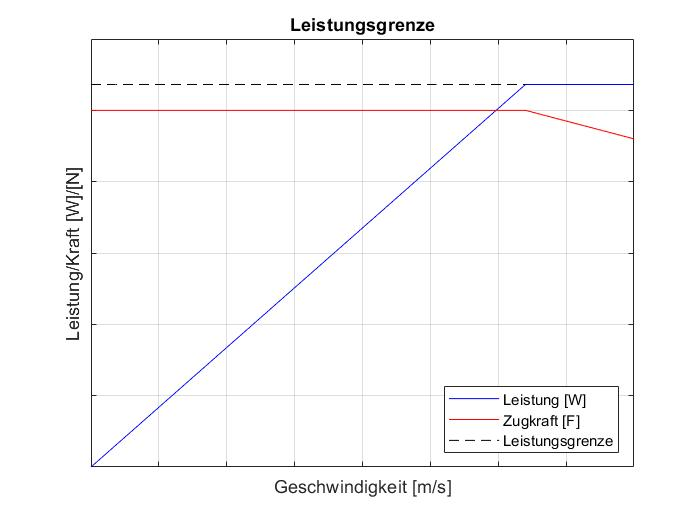
\includegraphics[width=1\linewidth]{LeistungKraft.jpg}
	\caption{Leistungsgrenze}\label{fig:LeistungKraft}
\end{figure}

Diese Leistungsgrenze ist abhängig von der Energieversorgung. Da diese mit Batterien realisiert wird, ist der Innenwiderstand der Batterie ein wichtiger Faktor. Zudem hat der Ladezustand einen Einfluss darauf, da die Spannung der Batterie beim entladen dieser abnimmt.\\
Die Temperatur-Versuche haben zudem aufgezeigt, dass sowohl der Motor als auch die Ansteuerung gekühlt werden müssen, da diese ansonsten überhitzen. Vor allem im Abrollbetrieb, wenn ein höheres Intervall gefahren werden kann, ist die Kühlung des Motors enorm wichtig.\\

Anhand der Versuche konnte bewiesen werden, dass der Motor alle Anforderungen für den Einzugswindenbetrieb erfüllt. Die effektive maximale Leistung hängt jedoch von der Energieversorgung ab. Da diese wiederum vom Innenwiderstand, dem Batterietyp und dem Ladezustand abhängt, kann eine definitive Aussage über die max. Leistung erst beim fertigen Aufbau gemacht werden.